\section{Cortando o Papel}

\begin{frame}[fragile]{Problema}

Uma folha de papel é composta de uma sequência de retângulos com diferentes alturas mas com
larguras fixas, tal que as bases dos retângulos estão assentadas em uma linha horizontal. A figura
ilustra uma folha exemplo com 33 retângulos. Nós gostaríamos de fazer um único corte horizontal,
com a ajuda de um estilete e uma régua, que maximize o número resultante de pedaços separados pelo
corte. A figura mostra quatro diferentes cortes que resultariam, respectivamente, em 4, 11, 10 e 3
pedaços.

\end{frame}


\begin{frame}[fragile]{Problema}
    \begin{figure}[!ht]
        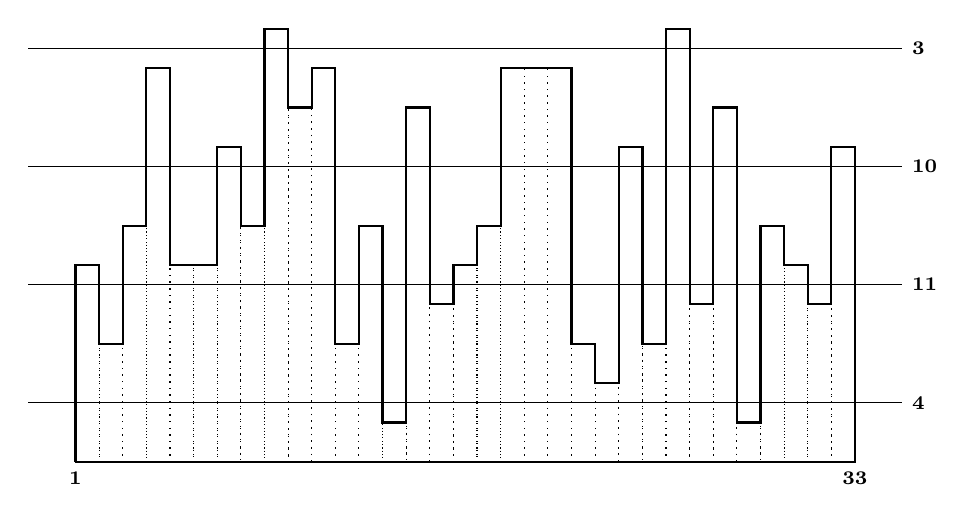
\begin{tikzpicture}

\draw[dotted] (0.0, 0) rectangle (0.3, 2.5);
\draw[dotted] (0.3, 0) rectangle (0.6, 1.5);
\draw[dotted] (0.6, 0) rectangle (0.8999999999999999, 3.0);
\draw[dotted] (0.8999999999999999, 0) rectangle (1.2, 5.0);
\draw[dotted] (1.2, 0) rectangle (1.5, 2.5);
\draw[dotted] (1.5, 0) rectangle (1.8, 2.5);
\draw[dotted] (1.8, 0) rectangle (2.1, 4.0);
\draw[dotted] (2.1, 0) rectangle (2.4, 3.0);
\draw[dotted] (2.4, 0) rectangle (2.6999999999999997, 5.5);
\draw[dotted] (2.6999999999999997, 0) rectangle (2.9999999999999996, 4.5);
\draw[dotted] (2.9999999999999996, 0) rectangle (3.2999999999999994, 5.0);
\draw[dotted] (3.2999999999999994, 0) rectangle (3.599999999999999, 1.5);
\draw[dotted] (3.599999999999999, 0) rectangle (3.899999999999999, 3.0);
\draw[dotted] (3.899999999999999, 0) rectangle (4.199999999999999, 0.5);
\draw[dotted] (4.199999999999999, 0) rectangle (4.499999999999999, 4.5);
\draw[dotted] (4.499999999999999, 0) rectangle (4.799999999999999, 2.0);
\draw[dotted] (4.799999999999999, 0) rectangle (5.099999999999999, 2.5);
\draw[dotted] (5.099999999999999, 0) rectangle (5.399999999999999, 3.0);
\draw[dotted] (5.399999999999999, 0) rectangle (5.699999999999998, 5.0);
\draw[dotted] (5.699999999999998, 0) rectangle (5.999999999999998, 5.0);
\draw[dotted] (5.999999999999998, 0) rectangle (6.299999999999998, 5.0);
\draw[dotted] (6.299999999999998, 0) rectangle (6.599999999999998, 1.5);
\draw[dotted] (6.599999999999998, 0) rectangle (6.899999999999998, 1.0);
\draw[dotted] (6.899999999999998, 0) rectangle (7.1999999999999975, 4.0);
\draw[dotted] (7.1999999999999975, 0) rectangle (7.499999999999997, 1.5);
\draw[dotted] (7.499999999999997, 0) rectangle (7.799999999999997, 5.5);
\draw[dotted] (7.799999999999997, 0) rectangle (8.099999999999998, 2.0);
\draw[dotted] (8.099999999999998, 0) rectangle (8.399999999999999, 4.5);
\draw[dotted] (8.399999999999999, 0) rectangle (8.7, 0.5);
\draw[dotted] (8.7, 0) rectangle (9.0, 3.0);
\draw[dotted] (9.0, 0) rectangle (9.3, 2.5);
\draw[dotted] (9.3, 0) rectangle (9.600000000000001, 2.0);
\draw[dotted] (9.600000000000001, 0) rectangle (9.900000000000002, 4.0);
\draw (-0.6, 0.75) -- (10.500000000000002, 0.75) node[anchor=west] { \scriptsize \bf 4 };
\draw (-0.6, 2.25) -- (10.500000000000002, 2.25) node[anchor=west] { \scriptsize \bf 11 };
\draw (-0.6, 3.75) -- (10.500000000000002, 3.75) node[anchor=west] { \scriptsize \bf 10 };
\draw (-0.6, 5.25) -- (10.500000000000002, 5.25) node[anchor=west] { \scriptsize \bf 3 };
\node[anchor=north] at (0, 0) { \scriptsize \bf 1 };
\node[anchor=north] at (9.900000000000002, 0) { \scriptsize \bf 33 };
\draw[thick] (0, 0) -- (0.0, 2.5) -- (0.3, 2.5) -- (0.3, 1.5) -- (0.6, 1.5) -- (0.6, 3.0) -- (0.8999999999999999, 3.0) -- (0.8999999999999999, 5.0) -- (1.2, 5.0) -- (1.2, 2.5) -- (1.5, 2.5) -- (1.5, 2.5) -- (1.8, 2.5) -- (1.8, 4.0) -- (2.1, 4.0) -- (2.1, 3.0) -- (2.4, 3.0) -- (2.4, 5.5) -- (2.6999999999999997, 5.5) -- (2.6999999999999997, 4.5) -- (2.9999999999999996, 4.5) -- (2.9999999999999996, 5.0) -- (3.2999999999999994, 5.0) -- (3.2999999999999994, 1.5) -- (3.599999999999999, 1.5) -- (3.599999999999999, 3.0) -- (3.899999999999999, 3.0) -- (3.899999999999999, 0.5) -- (4.199999999999999, 0.5) -- (4.199999999999999, 4.5) -- (4.499999999999999, 4.5) -- (4.499999999999999, 2.0) -- (4.799999999999999, 2.0) -- (4.799999999999999, 2.5) -- (5.099999999999999, 2.5) -- (5.099999999999999, 3.0) -- (5.399999999999999, 3.0) -- (5.399999999999999, 5.0) -- (5.699999999999998, 5.0) -- (5.699999999999998, 5.0) -- (5.999999999999998, 5.0) -- (5.999999999999998, 5.0) -- (6.299999999999998, 5.0) -- (6.299999999999998, 1.5) -- (6.599999999999998, 1.5) -- (6.599999999999998, 1.0) -- (6.899999999999998, 1.0) -- (6.899999999999998, 4.0) -- (7.1999999999999975, 4.0) -- (7.1999999999999975, 1.5) -- (7.499999999999997, 1.5) -- (7.499999999999997, 5.5) -- (7.799999999999997, 5.5) -- (7.799999999999997, 2.0) -- (8.099999999999998, 2.0) -- (8.099999999999998, 4.5) -- (8.399999999999999, 4.5) -- (8.399999999999999, 0.5) -- (8.7, 0.5) -- (8.7, 3.0) -- (9.0, 3.0) -- (9.0, 2.5) -- (9.3, 2.5) -- (9.3, 2.0) -- (9.600000000000001, 2.0) -- (9.600000000000001, 4.0) -- (9.900000000000002, 4.0) -- (9.900000000000002, 0) -- (0, 0);

        \end{tikzpicture}
    \end{figure}
\end{frame}



\begin{frame}[fragile]{Entrada e saída}

\textbf{Entrada}

A primeira linha da entrada contém um inteiro $N$, representando o número de retângulos na folha de
papel. A segunda linha contém $N$ inteiros $A_i$, $1\leq i\leq N$, representando a sequência de
alturas dos retângulos.

\vspace{0.1in}

\textbf{Saída}

Seu programa deve imprimir uma linha contendo um inteiro representando o número máximo de pedaços
possível, com um único corte horizontal.

\end{frame}

\begin{frame}[fragile]{Entrada e saída}

\textbf{Restrições}

\begin{itemize}
    \item $2\leq N\leq 10^5$
    \item $1\leq A_i\leq 10^9$, para $1\leq i\leq N$
\end{itemize}

\vspace{0.1in}

\textbf{Informações sobre a pontuação}

\begin{itemize}
    \item Em um conjunto de casos de teste somando 40 pontos, $N\leq 1000$
\end{itemize}
\end{frame}

\begin{frame}[fragile]{Exemplo de entradas e saídas}

\begin{minipage}[t]{0.45\textwidth}
\textbf{Entrada}
\begin{verbatim}
5 6
1 2 4
1 3 3
4 3 6
4 5 2
2 4 1
3 5 5
\end{verbatim}
\end{minipage}
\begin{minipage}[t]{0.5\textwidth}
\textbf{Saída}
\begin{verbatim}
7
\end{verbatim}
\end{minipage}
\end{frame}

\begin{frame}[fragile]{Exemplo de entradas e saídas}

\begin{minipage}[t]{0.45\textwidth}
\textbf{Entrada}
\begin{verbatim}
7 10
1 2 5
3 1 32
1 4 3
2 3 4
2 6 20
6 3 1
6 4 9
6 5 6
3 7 18
5 7 2
\end{verbatim}
\end{minipage}
\begin{minipage}[t]{0.5\textwidth}
\textbf{Saída}
\begin{verbatim}
18
\end{verbatim}
\end{minipage}
\end{frame}


\begin{frame}[fragile]{Solução}

    \begin{itemize}
        \item Uma parte importante do problema consiste em identificar o número de pedaços 
            resultantes de um corte na altura $x$

        \item Conforme pode ser observado na figura, um pedaço consiste em uma série de retângulos
            contíguos cujas alturas são todas maiores do que $x$

        \item Além disso, há o pedaço formado por todos os retângulos, ou partes de retângulo,
            que ficaram abaixo de $x$

        \item É possível usar a técnica de dois ponteiros para identificar os pedaços resultantes
            de um corte em $x$
    \end{itemize}

\end{frame}

\begin{frame}[fragile]{Rotina que computa os pedaços para um corte em $x$}
    \inputsnippet{cpp}{1}{21}{codes/corte.cpp}
\end{frame}

\begin{frame}[fragile]{Solução}

    \begin{itemize}
        \item A rotina $pieces(x)$, que computa o número de pedaços resultantes de um corte em 
            $x$, tem complexidade $O(N)$

        \item Uma solução para o problema consiste em computar o valor máximo de $pieces(x)$
            para $x \in [1, M]$, onde $M = \max\{ h_1, h_2, \ldots,
            h_N\}$

        \item Tal solução tem complexidade $O(NM)$, e como $N\leq 10^5$ e $M\leq 10^9$, tal 
            abordagem resulta em um veredito TLE
    \end{itemize}

\end{frame}

\begin{frame}[fragile]{Solução TLE $O(MN)$}
    \inputsnippet{cpp}{1}{21}{codes/papel_bf.cpp}
\end{frame}

\begin{frame}[fragile]{Solução TLE $O(MN)$}
    \inputsnippet{cpp}{22}{42}{codes/papel_bf.cpp}
\end{frame}

\begin{frame}[fragile]{Solução TLE $O(MN)$}
    \inputsnippet{cpp}{43}{63}{codes/papel_bf.cpp}
\end{frame}

\begin{frame}[fragile]{Solução}

    \begin{itemize}
        \item Por meio de uma observação cuidadosa dos cortes para valores consecutivos de $x$ 
            leva a conclusão que os valores de $pieces(x)$ só se modificam nos valores que
            correspondem às alturas dos retângulos

        \item Isto reduz a quantidade máxima de alturas a serem verificadas de $10^9$ para $10^5$

        \item Embora o veredito continue sendo TLE, esta redução permite resolver com sucesso o
            conjunto de casos de testes que correspondem a 40 pontos

        \item Para somar todos os 100 pontos, é preciso uma abordagem distinta que identifique,
            de forma eficiente, os valores de $x$ que levam aos cortes com o número máximo de
            pedaços
    \end{itemize}

\end{frame}

\begin{frame}[fragile]{Solução}

    \begin{itemize}
        \item Considere a figura abaixo

        \begin{figure}
    \centering

    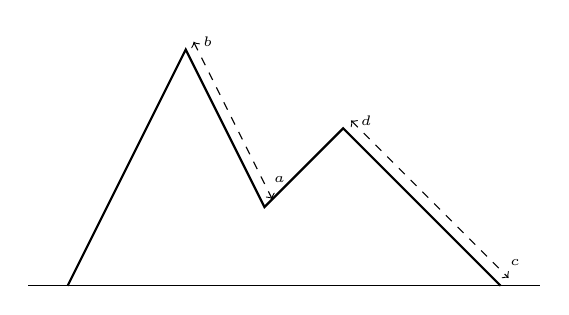
\begin{tikzpicture}[scale=0.5]
        \draw (0, 2) -- (13, 2);
        \draw[thick] (1, 2) -- (4, 8) -- (6, 4) -- (8, 6) -- (12, 2);

        \draw[<->, dashed] (4.2, 8.2) -- (6.2, 4.2);
        \draw[<->, dashed] (8.2, 6.2) -- (12.2, 2.2);
        \node[anchor=west] at (4.2, 8.2) {\tiny $b$ };
        \node[anchor=west] at (6.0, 4.7) {\tiny $a$ };
        \node[anchor=west] at (8.2, 6.2) {\tiny $d$ };
        \node[anchor=west] at (12.0, 2.6) {\tiny $c$ };
    \end{tikzpicture}

\end{figure}


        \item Um corte com $x\in [a, b)$ divide o primeiro pico em duas partes

        \item Já um corte com $x \in [c, d)$ divide o segundo pico em duas partes

    \end{itemize}

\end{frame}


\begin{frame}[fragile]{Solução}

    \begin{itemize}
        \item Agora, se $x\in [a, b)\cap [c, d)$, ambos serão divididos

        \item Considerando que o $i$-ésimo pico pode ser caracterizado por um ponto de máximo local
            $b_i$ e um ponto de mínimo local $a_i$, o problema passa a ser determinar a maior
            interseção possível entre todos os intervalos $[a_i, b_i)$
            
        \item Para identificar de forma mais simples e eficiente os pontos de máximo e mínimo
            locais, a entrada pode ser comprimida, eliminando-se alturas iguais e consecutivas:

            \vspace{0.1in}

            \inputsyntax{cpp}{codes/compress.cpp}
    \end{itemize}

\end{frame}

\begin{frame}[fragile]{Solução}

    \begin{itemize}
        \item Após a compressão, há um ponto de máximo local em $h_i$ se $h_{i - 1} < h_i$ e
            $h_{i + 1} < h_i$

        \item De forma análoga, há um ponco de mínimo local em $h_i$ se $h_{i - 1} > h_i$ e
            $h{i + 1} > h_i$

        \item Por fim, a maior interseção possível entre todos os intervalos $[a_i, b_i)$ pode
            ser determinada por meio de um algoritmo de \textit{line sweep}

        \item Para cada intervalo $a_i$ deve ser criados dois eventos: um evento de abertura em
            $a_i$ e um e fechamento em $b_i$

        \item Os eventos devem ser ordenados pelo ponto de ocorrência

        \item Em caso de empate, os eventos de fechamento devem vir antes dos de abertura

    \end{itemize}

\end{frame}

\begin{frame}[fragile]{Solução}

    \begin{itemize}
        \item Os eventos devem ser processados em ordem

        \item Inicialmente não há nenhum intervalo aberto

        \item Cada abertura incrementa em uma unidade o número de intervalos abertos

        \item Os eventos de fechamento reduzem o número de intervalos abertos em uma unidade

        \item A solução do problema é o maior número de intervalos abertos registrado durante
            o processamento dos eventos

        \item Assim, como a compressão tem complexidade $O(N)$ e a ordenação dos eventos
            $O(N\log N)$, a solução tem complexidade $O(N\log N)$
    \end{itemize}

\end{frame}
\begin{frame}[fragile]{Solução $O(N\log N)$}
    \inputsnippet{cpp}{1}{21}{codes/papel.cpp}
\end{frame}

\begin{frame}[fragile]{Solução $O(N\log N)$}
    \inputsnippet{cpp}{22}{42}{codes/papel.cpp}
\end{frame}

\begin{frame}[fragile]{Solução $O(N\log N)$}
    \inputsnippet{cpp}{43}{63}{codes/papel.cpp}
\end{frame}

